\chapter{Projektplan}
\section{Änderungsgeschichte}
\begin{tabularx}{\textwidth}{|c|c|X|c|}
  \hline
  \textbf{Datum} & \textbf{Version} & \textbf{Änderung} & \textbf{Autor} \\
  \hline \hline
  26.02.2016 & 1.0 & Erstellen des Projektplans & Martin Stypinski \\
  \hline
\end{tabularx}

\section{Einleitung}
\subsection{Ziel und Zweck}
Ziel dieser Arbeit ist \textit{Project-Helin} umzusetzten. 

\subsection{Lieferumfang}
Der Lieferumfang dieser Arbeit entspricht den Vorgaben der HSR:
\begin{itemize}
	\item{Zu Handen des Betreuers:
	\begin{itemize}
		\item{Ein gedrucktes Exemplar der Dokumentation}
		\item{Dokumentation, sämtliche Dokumente und Sourcen auf CD}
	\end{itemize}}
	\item{Poster - Enthält Zusammenfassung der Arbeit}
	\item{Abstract für die Bachelorarbeitsbrochure}
\end{itemize}
Zusätzlich ist es uns ein Anliegen, dass der Sourcecode und die Erfahrungen über den Zeitraum der Bachelorarbeit hinaus bestehen bleiben. Daher wurde ein github-repository eingerichtet, dass nach beendigung der Arbeit sämtliche Teile enthält: \textbf{\url{https://github.com/Project-Helin}}

\subsection{Annahmen und Einschränkungen}
Es kann angenommen werden, dass der Zeitplan im Rahmen der regulären Bachelorarbeit Zeit gültig ist. Es wird dabei berücksichtigt das ein Zeithorizont von 17 Wochen zuverfügung steht und die maximale Arbeitszeit von 360 Stunden pro Person nicht überschritten werden soll.

\newpage

\section{Projektorganisation}
\subsection{Organisationsstruktur}

\begin{figure}[ht]
%\begin{figure}[H]
	\centering
	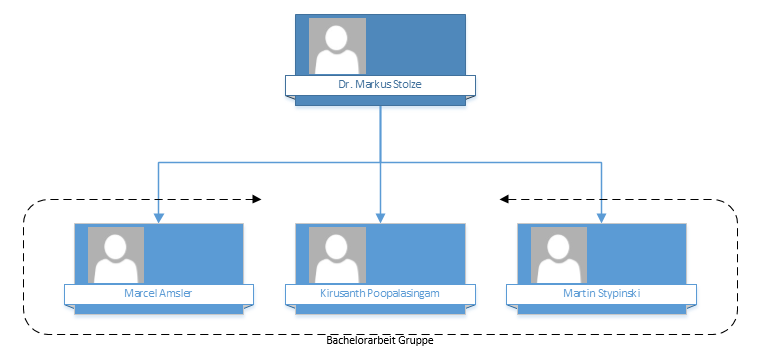
\includegraphics[width=\textwidth]{images/organigram.png}
	\caption{Grobübersicht über den Projektplan}
	\label{Risk result}
\end{figure}

\begin{tabularx}{\textwidth}{|c|c|X|}
  \hline
  \textbf{Name} & \textbf{E-Mail} & \textbf{Verantwortung} \\
  \hline \hline
  Prof. Dr. Markus Stolze & \url{markus.stolze@hsr.ch} & Betreuer der Arbeit\\
  \hline \hline
  Marcel Amsler & \url{marcel.amsler@hsr.ch} & \\
  \hline
  Kirusanth Poopolasingam & \url{kirusanth.poopalasingam@hsr.ch} & \\
  \hline
  Martin Stypinski & \url{martin.stypinski@hsr.ch} & \\
    \hline
\end{tabularx}

\newpage

\section{Meilensteinplanung}
Grundsätzlich wird während der gesammten Arbeit Scrum als Projektmanagement eingsetzt. Ein Scrum-Sprint dauer in der Regel 2 Wochen. Die Meilensteine helfen nur zu definieren welche Tasks prioritär behandelt werden sollen.

\begin{figure}[ht]
%\begin{figure}[H]
	\centering
	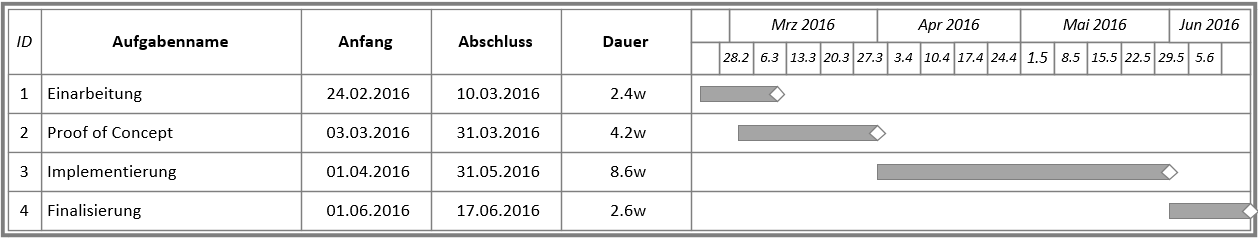
\includegraphics[width=\textwidth]{images/projplan.png}
	\caption{Grobübersicht über den Projektplan}
	\label{Risk result}
\end{figure}


\begin{itemize}
	\item{\textbf{Ende der Einarbeitung:} 
		\begin{itemize}
			\item{\textbf{Datum:} 10.03.2015}
			\item{\textbf{Ziel:} Entwicklungsumgebund und Prozesse stehen.}
			\item{\textbf{Erfüllungskriterium:} Sämtliche prozessbegleitenden Massnahmen sind lauffähig. Projektmanagement-Tool, IDEs, CI}
		\end{itemize}
	}
	
	\item{\textbf{Ende des Proof of Concept:} 
		\begin{itemize}
			\item{\textbf{Datum:} 31.03.2015}
			\item{\textbf{Ziel:} Die Machbarkeit ist bewiesen.}
			\item{\textbf{Erfüllungskriterium:} Prototyp ist lauffähig, zeigt Machbarkeit und allfällige Einschränkungen.}
		\end{itemize}
	}
	
	\item{\textbf{Ende der Implementierung:} 
		\begin{itemize}
			\item{\textbf{Datum:} 27.05.2015}
			\item{\textbf{Ziel:} Code Freeze}
			\item{\textbf{Erfüllungskriterium:} Alle zwingenden funktionalen- und nicht-funktionalen Anforderungen sind erfüllt.}
		\end{itemize}
	}	
	\item{\textbf{Abgabe} 
			\begin{itemize}
				\item{\textbf{Datum:} 17.06.2015}
				\item{\textbf{Ziel:} Abgabe der Arbeit}
				\item{\textbf{Erfüllungskriterium:} Alle im Lieferumfang geforderten Dokumente sind fertiggestellt.}
			\end{itemize}
	}
	
\end{itemize}

\newpage

\section{Risikomanagement}
\subsection{Risiken}
\LTXtable{\textwidth}{risk.tex}

\subsection{Umgang mit Risiken}
Die Risken wurden in einer Risiko Matrix aufgegliedert umd besser zu verstehen welche Risiken eine grosse Bedrohung bringen.

\begin{figure}[ht]
%\begin{figure}[H]
	\centering
	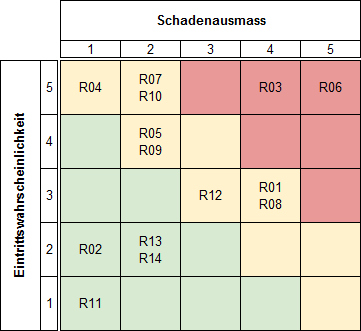
\includegraphics[scale=0.7]{images/risk_result.png}
	\caption{Risiko Matrix}
	\label{Risk result}
\end{figure}

Als Konsequenz kann folgende Aufteilung getroffen werden:
\begin{itemize}
	\item{\textbf{Risiko hoch: } R03, R06}
	\item{\textbf{Risiko mittel:} R01, R04, R05, R07, R08, R09, R10, R12 }
	\item{\textbf{Risiko klein:} R02, R11, R13, R14}
\end{itemize}
\subsection{Massnahmen}
Für die hohen und mittleren Risiken wurden folgende Massnahmen festgelegt:
\begin{itemize}
	\item{\textbf{R03 - Internet auf Mobilgerät:} \\
	\textbf{Massnahmen:} Es muss sichergestellt werden, dass die Drohne nicht auf eine permanente Serververbindung angewiesen ist. Monitor und Datenlogging dürfen kurze Unterbrechungen aufweisen. Die Mission darf aber zu keinem Zeitpunkt gefährdet werden, die Drohne muss selbstständig am Bestimmungsort landen.}
	
	\item{\textbf{R06 - Absturz und Schäden:} \\
	\textbf{Massnahmen:} Bei der Wahl der Drohne wurde auf eine Verfügbarkeit der Ersatzteile geachtet. Ebenfalls wurde darauf geachtet, dass die Bezugsquellen in der Schweiz einen adequaten Lagerbestand aufweisen.}

	\item{\textbf{R01 - JMS auf Mobilgerät:} \\
	\textbf{Massnahmen:} Bei der Evaluierung der Komponenten wird ein JMS Implementierung gewählt, die auf einem Android Betriebssystem lauffähig ist. Dies wird in einem Proof of Concept überprüft.}
	
	\item{\textbf{R04 - Infrastruktur Problme:} \\
	\textbf{Massnahmen:} Auf Grund von Erfahrungen aus früheren Projekten, wird auf die Serverinfrastruktur der HSR verzichtet, dies garantiert eine volle Kontrolle über den Server. Es muss jedoch berücksichtig werden, dass der administrativ Aufwand höher ist und somit mehr Zeit in Anspruch nehmen wird.}
	
	\item{\textbf{R05 - Kapazität der Drohne:} \\
	\textbf{Massnahmen:} Sollte die Drohne nicht ein Gewicht transportieren, dass einer Demonstration würdig ist, wird ein Akkupack mit mehr Spannung angeschaft.}	
	
	\item{\textbf{R07 - Positionsungenauigkeit:} \\
	\textbf{Massnahmen:} Bei Flugkoridoren und Landepunkten genügend Sicherheitsmarge einrechnen, damit die GPS Ungenauigkeit keine unvorhergesehnen Probleme bereiten kann.}
	
	\item{\textbf{R08 - Ardupilot Handhabung:} \\
	\textbf{Massnahmen:} Von Anfang an die gesammte Route an Ardupilot übertragen. Dies muss in einem Proof of Concept genauer eruiert werden.}
	
	\item{\textbf{R09 - Ardupilot API:} \\
	\textbf{Massnahmen:} Früh in einem Proof of Concept die Möglichkeiten und Grenzen des APIs nachvollziehen.}
	
	\item{\textbf{R10 - Entwicklungsprozesse:} \\
	\textbf{Massnahmen:} Bewusster Umgang mit der Resource Zeit. Gegebenenfalls Arbeitsplatz im Freien, um Zeit während des Deployments auf die Drohne zu sparen.}
	
	\item{\textbf{R12 - Ablademanagement:} \\
	\textbf{Massnahmen:} Prüfung einer Abwurfmöglichkeit. Gegebenenfalls Benutzer mit GUI auf Mobile begleiten um einen sicheren und unfallfreien Ablad zu garantieren.}
\end{itemize}

\section{Qualitätsmassnahmen}	
\subsection{Dokumentation}
Die Dokumentation wird vollständig in Latex geschrieben und befindet sich zu jedem Zeitpunkt auf dem Project-Helin github repository: github.com/project-helin.

\subsection{Projektmanagement}
Für das Projektmanagement wird Jira von Atlassian verwendet. \\
Als Projektmanagmenet Methodik wird Scrum verwendet, jedoch werden einige Meilensteine gesetzt um den Fokus nicht aus den Augen zu verlieren und sich über Teilziele bewusst zu sein.

\subsection{Entwicklung}
Die Qualität der Entwicklung wird durch folgende Massnahmen sichergestellt:
\begin{itemize}
	\item{\textbf{Code Review:} Bei kritischen Komponenten werden Code Reviews durchgeführt um sich Designentscheidungen bewusst vor Augen zu führen.}
	
	\item{\textbf{Testing:} Das gesammte Projekt wird in Java entwickelt. Als Unit-Test Framework wird folglich JUnit4 verwendet.}
	
	\item{\textbf{Versionierung:} Der gesammte Quellcode wird mithilfe von github versioniert.}
	
	\item{\textbf{Deployment:} Die Serverkomponenten werden mithilfe eines Build Systems deployt. Die Komponenten auf den Mobiltelefonen werden manuell deployt. Jedoch werden auf dem Build-System ebenfalls Unit-Tests zu Verfügung gestellt.}
	
\end{itemize}